\begin{frame}{Arquitectura del motor sistema oscillador}
    \centering
    \begin{columns}
        \begin{column}{0.75\textwidth}
            \begin{figure}
                \centering
            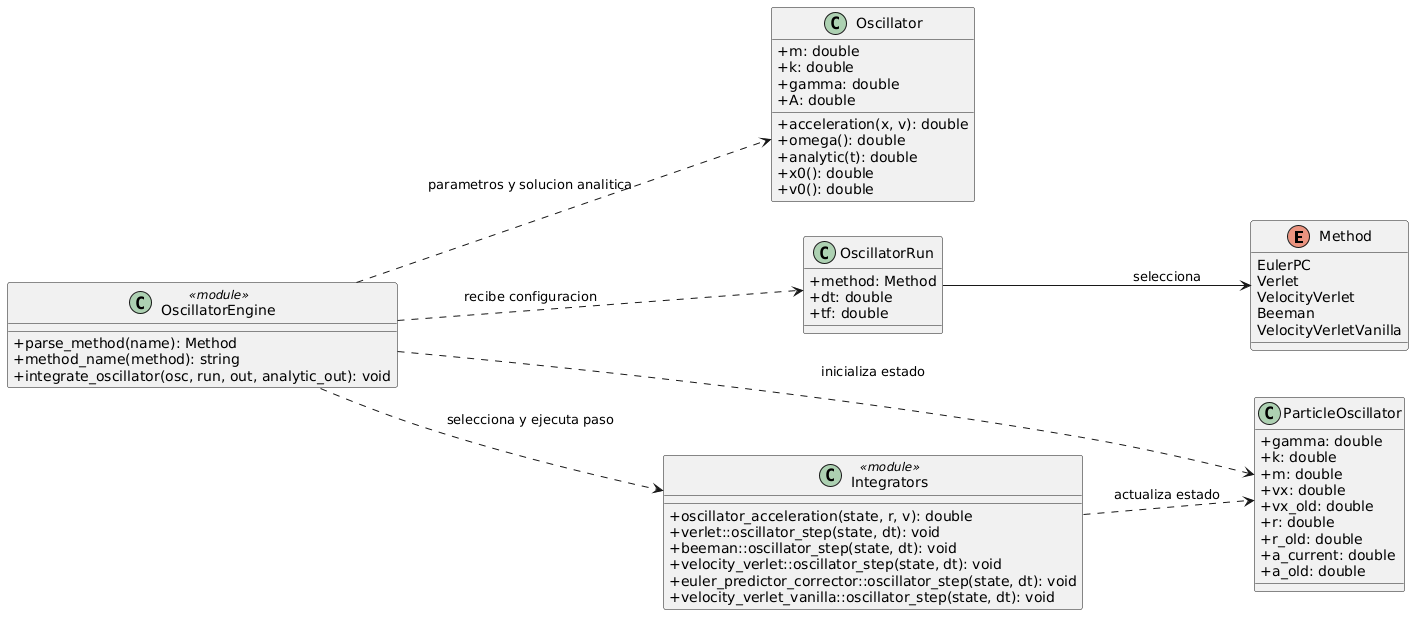
\includegraphics[width=1\linewidth]{uml_simple_oscillator.png}
            \end{figure}
        \end{column}
        \begin{column}{0.25\textwidth}
            \begin{itemize}
                \item Motor hecho en C++
            \end{itemize}
        \end{column}
    \end{columns}
\end{frame}

\begin{frame}{Velocity Verlet Modificado}


\end{frame}

\begin{frame}{$F_u$ en función de la densidad con corte a $t = 30$}
  \begin{cols}
    \begin{column}{0.62\textwidth}
      \figura{fu30_vs_phi.png}
    \end{column}
    \begin{column}{0.34\textwidth}
      \begin{parametros}
        \item $x_o = r$
        \item $10$ realizaciones
      \end{parametros}
    \end{column}
  \end{cols}
\end{frame}
